\documentclass[11pt,a4paper]{article}
\usepackage[margin=2.5cm]{geometry}
\usepackage{graphicx}
\usepackage{float}

\title{Report 6: Map}
\author{Le Nguyen Minh Quang (2540093)}
\date{\today}

\begin{document}
\maketitle

\section{What is Map}
From the slides, Map is the simplest parallel pattern:
\begin{itemize}
  \item We apply the same function f to every element of an array.
  \item Each output only depends on one input. We do not need the
  neighbours.
  \item There is a one to one relationship between input and output.
  \item Because of this, it is very easy to run in parallel and we can
  get almost linear speedup.
\end{itemize}
On the GPU, one thread handles one element:
\begin{verbatim}
def kernel(src, dst):
    tid = ...
    dst[tid] = f(src[tid])
\end{verbatim}
In this labwork, one element is one pixel. I use 2D blocks like in
labwork 4, so each thread finds its pixel with tidx and tidy and
applies f to it.

I ran the code on Google Colab with a Tesla T4 GPU. My image is
1200x750 pixels.

\section{6a: Binarization}
First I convert the image to gray with my grayscale kernel from
labwork 4. Then every gray pixel becomes black or white using a
threshold. I used threshold = 128. If the pixel is smaller than 128 it
becomes 0 (black), otherwise it becomes 255 (white). I used 255 instead
of 1 so we can see the image.
\begin{verbatim}
if src[tidy, tidx] < threshold:
    dst[tidy, tidx] = 0
else:
    dst[tidy, tidx] = 255
\end{verbatim}

\section{6b: Brightness control}
To make the image brighter I add a value to every pixel (for each
colour R, G, B). A negative value makes it darker. I used value = 80.
The result must stay between 0 and 255, so I cut it.
\begin{verbatim}
for ch in range(3):
    v = src[tidy, tidx, ch] + value
    if v > 255:
        v = 255
    if v < 0:
        v = 0
    dst[tidy, tidx, ch] = v
\end{verbatim}

\section{6c: Blending two images}
Blending mixes two images of the same size with a weight c:
\[
Q(x, y) = c \cdot image1(x, y) + (1 - c) \cdot image2(x, y)
\]
For the second image I flipped my image left to right, so both images
have the same size. I used c = 0.5, so both images count the same.
\begin{verbatim}
for ch in range(3):
    p1 = src1[tidy, tidx, ch]
    p2 = src2[tidy, tidx, ch]
    dst[tidy, tidx, ch] = np.uint8(c * p1 + (1 - c) * p2)
\end{verbatim}

\section{Results}
\begin{figure}[H]
  \centering
  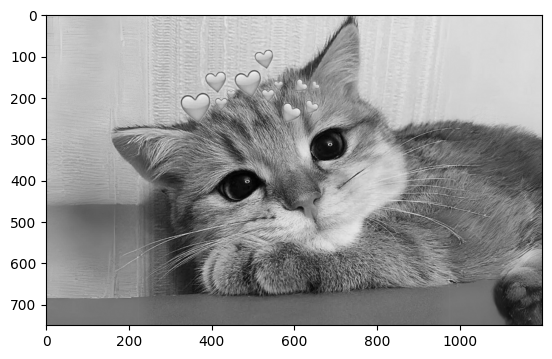
\includegraphics[width=0.48\textwidth]{gray.png}
  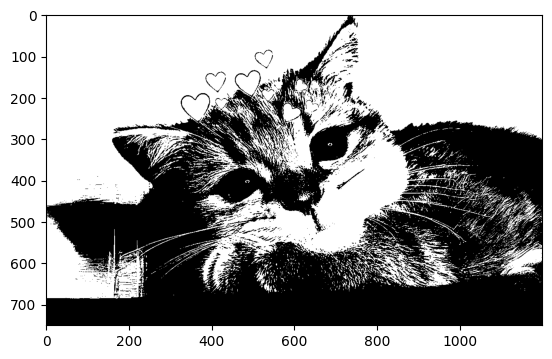
\includegraphics[width=0.48\textwidth]{binary.png}
  \caption{Gray image (left) and binarization with threshold 128
  (right).}
\end{figure}

\begin{figure}[H]
  \centering
  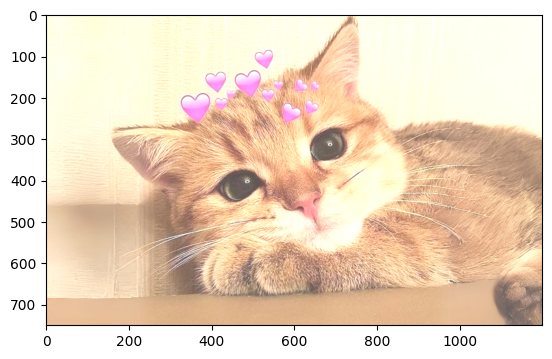
\includegraphics[width=0.48\textwidth]{bright.png}
  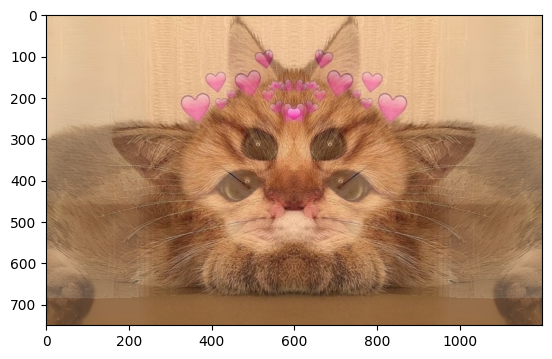
\includegraphics[width=0.48\textwidth]{blend.png}
  \caption{Brightness +80 (left) and blending with c = 0.5 (right).}
\end{figure}

\section{Block size experiment}
I tried 4 block sizes. One kernel call is very short, so I ran each
kernel 50 times and took the average time.

\begin{center}
\begin{tabular}{|c|c|c|c|}
\hline
Block & Binarization & Brightness & Blending \\ \hline
4x4   & 0.180 ms & 0.162 ms & 0.716 ms \\ \hline
8x8   & 0.044 ms & 0.090 ms & 0.362 ms \\ \hline
16x16 & 0.038 ms & 0.065 ms & 0.360 ms \\ \hline
32x32 & 0.042 ms & 0.077 ms & 0.397 ms \\ \hline
\end{tabular}
\end{center}

\begin{figure}[H]
  \centering
  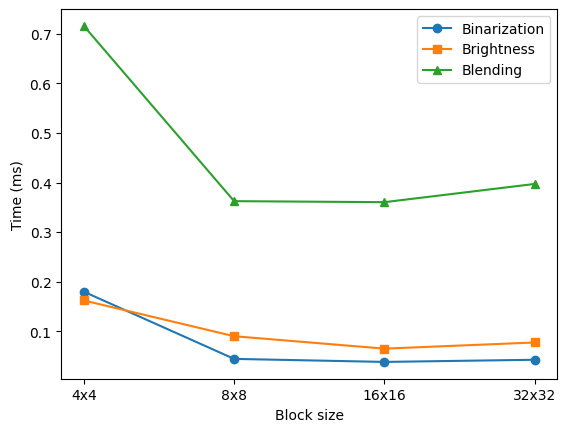
\includegraphics[width=0.7\textwidth]{blocksize_vs_time.png}
  \caption{Block size vs time.}
\end{figure}

What I see:
\begin{itemize}
  \item 4x4 is the slowest for all 3 kernels. A 4x4 block has only 16
  threads, but a warp has 32 threads, so half of the warp is not used.
  \item 16x16 is the fastest for all 3 kernels. 8x8 and 32x32 are
  almost as fast.
  \item Binarization is the fastest because it reads only 1 value per
  pixel (gray). Brightness reads 3 values (R, G, B).
  \item Blending is the slowest. It reads two images, so it reads twice
  as much memory. It also uses decimal numbers (c = 0.5), and I think
  this is slower on the GPU than integer math.
\end{itemize}

\section{Conclusion}
I implemented 3 map kernels: binarization, brightness control and
blending. They all follow the same idea from the slides: one thread
takes one pixel and applies a function to it. The best block size for
my image is 16x16, and blocks smaller than one warp (4x4) are slow.

\end{document}
